\subsubsection{Stern-Gerlach Experiment}

\begin{framed}
\textbf{Slogan:}\\
Stern-Gerlach demonstrated that the spin angular momentum of electron is quantized, with numerical values $\pm \hbar /2$
\end{framed}

Consider the following experimental set up:

\begin{figure}[!htbp]
\centering
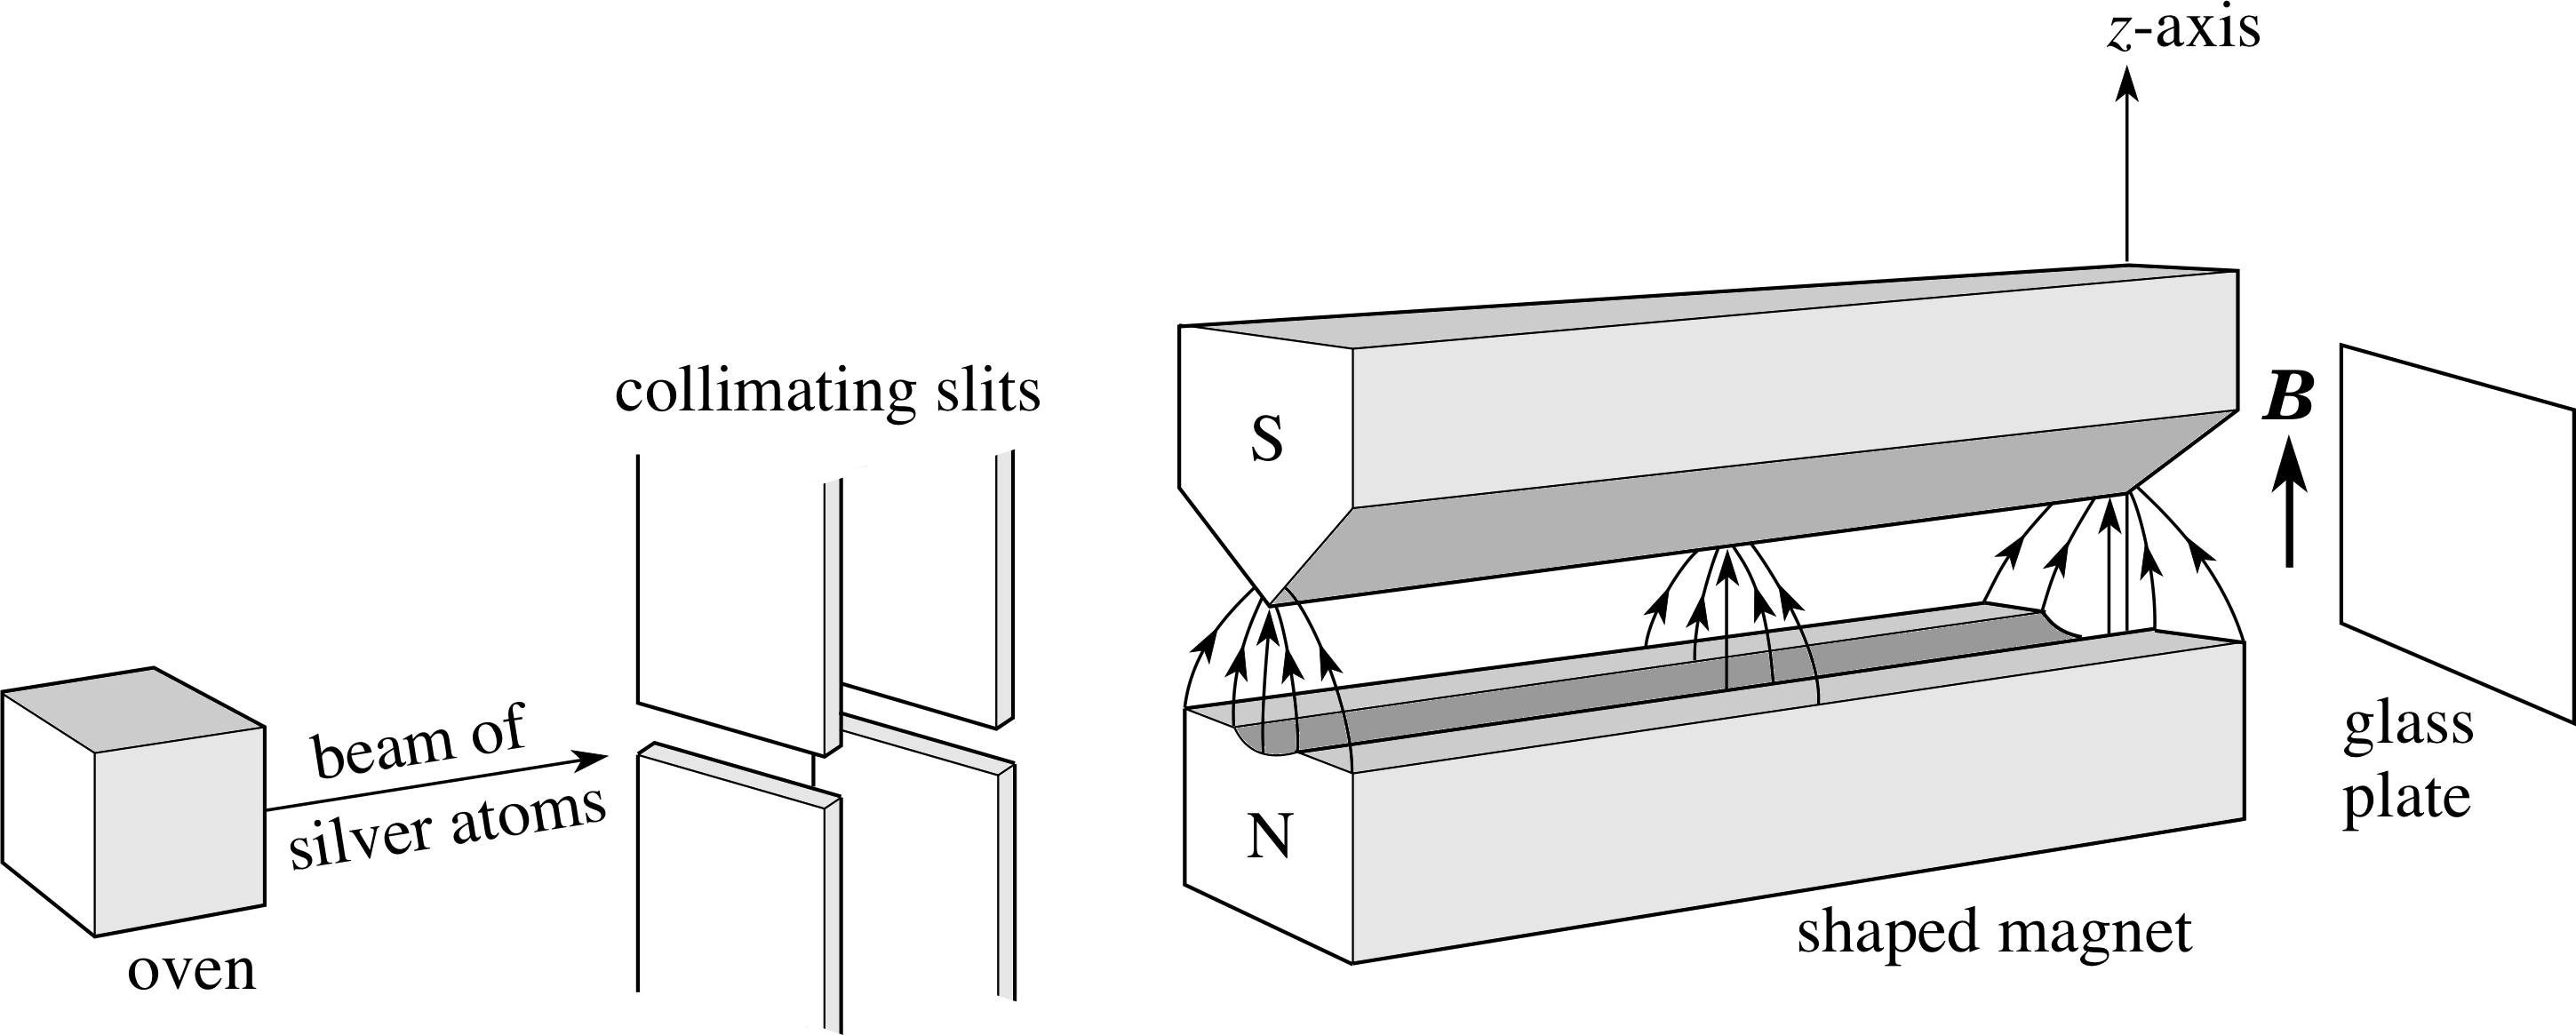
\includegraphics[width=0.7\linewidth]{files/S_G_experiment-437e0363a97a3f51196848de1f7c3d55.png}
\end{figure}

We want to know where would the silver atoms land on the glass plate. First we analyze through classical electromagnetics:

\begin{theorem}The potential energy of interaction between a \textbf{magnetic dipole}($\boldsymbol{\mu}$)and the \textbf{magnetic field}($\mathbf{B}$) is :
\begin{equation}
U = -\boldsymbol{\mu}\cdot \mathbf{B}
\end{equation}

\end{theorem}Since the energy is lowered if the dipole aligns with the magnetic field. As a result, the force experienced by the the dipole is simply:
\begin{equation}
\nabla U=-\nabla(\boldsymbol{\mu}\cdot \mathbf{B})
\end{equation}

In particular, we get that the $z$ component of the force is :

\begin{equation}
F^{(z)}&= -\partial_z (\mu^{(z)} B^{x}+ \mu^{(x)} B^{z} +\mu^{(y)} B^{y})
\end{equation}

In our case,